%
% File acl2019.tex
%
%% Based on the style files for ACL 2018, NAACL 2018/19, which were
%% Based on the style files for ACL-2015, with some improvements
%%  taken from the NAACL-2016 style
%% Based on the style files for ACL-2014, which were, in turn,
%% based on ACL-2013, ACL-2012, ACL-2011, ACL-2010, ACL-IJCNLP-2009,
%% EACL-2009, IJCNLP-2008...
%% Based on the style files for EACL 2006 by 
%%e.agirre@ehu.es or Sergi.Balari@uab.es
%% and that of ACL 08 by Joakim Nivre and Noah Smith

\documentclass[11pt,a4paper]{article}
\usepackage[hyperref]{acl2019}
\usepackage{times}
\usepackage{latexsym}
\usepackage{graphicx}
\graphicspath{ {./images/} }
\usepackage{algorithm}
\usepackage{algorithmic}
\usepackage{amsmath}
\DeclareMathOperator*{\argmax}{arg\,max}
\DeclareMathOperator*{\argmin}{arg\,min}
\usepackage{multirow}
\usepackage{float}
\usepackage{changepage}

% changed to avoid font problem
\usepackage[OT1]{fontenc} 

% Chinese support
\usepackage[UTF8]{ctex}

\usepackage{url}

\aclfinalcopy % Uncomment this line for the final submission
%\def\aclpaperid{***} %  Enter the acl Paper ID here

%\setlength\titlebox{5cm}
% You can expand the titlebox if you need extra space
% to show all the authors. Please do not make the titlebox
% smaller than 5cm (the original size); we will check this
% in the camera-ready version and ask you to change it back.

\newcommand\BibTeX{B\textsc{ib}\TeX}

\title{实验二:电商评论观点挖掘}

\author{
  牟虹霖 \\
  1173710132 \\
  \texttt{muhonglinyt@126.com} \\
  \\\And
  侯鹏钰 \\
  1173710217 \\
  \texttt{18800421656@163.com} \\
}

\date{}

\begin{document}
\maketitle
\begin{abstract}
  电商评论观点挖掘是当前电商平台分析消费者行为的关键内容之一,如何从海量的、文本类型复杂的评论中分析用户的兴趣和偏好,提取出用户关心的话题,
  以及满意和不满意的商品及其属性,是电商评论观点挖掘的重要任务。本文通过研究化妆品电商评论数据,实验传统统计模型\texttt{CRF}、深度学习模型\texttt{BiGRU-CRF}、
  预训练模型等完成命名实体识别问题、情感词属性词匹配问题、文本分类问题,分析各模型对电商评论观点数据挖掘的效果。

\end{abstract}

\begin{center}
  \large{\textbf{Abstract}}
\end{center}

\begin{adjustwidth}{0.6cm}{0.6cm}
  \fontsize{10pt}{12pt}
  E-commerce comment mining is one of the key contents of analyzing consumer behavior. 
  How to analyze user's interest and preference from massive and complex comments, extract user's concerned topics, 
  as well as satisfied and dissatisfied goods and their attributes, is an important task of e-commerce comment mining. 
  In this paper, using cosmetics e-commerce review data, we tried to solve the problems of named entity recognition, 
  opinion and aspect terms matching, text classification by experiencing traditional statistical model \texttt{CRF}, 
  deep learning model \texttt{BiGRU-CRF}, pre-training model and analyzed the effect of each model on e-commerce review data mining.
\end{adjustwidth}

% \keywords{电商观点评论, 命名实体识别, 文本分类}

\section{引言}
互联网技术和移动网络技术飞速发展的今天,电子商务和移动商务已经渗透到了生活的方方面面,电商平台上用户的行为分析已经变成企业进行消费者行为分析的重要组成部分。
电商评论数据作为大型电子商务平台上少有的可以被开放获得的用户行为数据,是进行用户行为分析的一个重要切入点,但电商平台的用户评论数据表现出了较强的大规模性、动态性和复杂性,且数据噪声较多,这些都成为研究本问题的难点。
本文将电商评论观点挖掘任务分为三个部分:属性词情感词抽取配对、属性分类和观点极性分类,上述三个任务分别被定义为NLP领域中的序列标注以及文本分类问题来实现。本文采用流水线的方式完成三部分的任务,任务定义如下:
\paragraph{属性词情感词抽取配对} 输入商品评论,输出为属性词以及对应的情感词
\paragraph{属性分类} 输入为第一部分得到的属性词情感词对,输出为属性词对应的类别,包括 \textit{包装},\textit{成分},\textit{尺寸},\textit{服务}等共13类
\paragraph{观点极性分类} 输入为第二部分得到的属性词情感词对以及分类信息,输出为该属性词情感词对的情感极性,包括\textit{正面},\textit{中性},\textit{负面}3类

% \section{问题定义}
% 分词问题的输入是一个字串:$ C=c_1,c_2,\cdots,c_n $ 输出是一个词串:$ S=w_1,w_2,\cdots,w_m $ ,其中要求 $ m \leq n $
% 对于一个特定的字符串$C$,会有多个切分方案$S$对应,最大概率分词就是在这些$S$中找出概率最大的一个切分方案,将其看作对于输入字符串切分的最有可能的词序列。

% \section{实验数据分析}

\section{相关工作}
本次实验中的细粒度情感分析主要包含属性词-情感词识别、属性词分类和观点极性分类。

属性词-情感词的抽取有基于频繁项集的算法,利用情感词和评价目标关系的方案,使用监督学习的做法和基于主题模型的方案。
频繁项集挖掘方法能够从给定领域的大量评论中找到显式的评价对象。\cite{hu2004mining}使用了频繁项集挖掘的方法。这种方法的缺点是要求评价对象的出现频率高,同时要求语料的相关性高。
因为情感词具有针对性,它们通常有一个所指向的评价目标。因而可以通过利用情感词和评价目标的关系来抽取属性词-情感词。\cite{hu2004mining}中采用了这种方法来抽取不常见的评价对象。
属性词-情感词的抽取还可以看作一般的信息抽取问题的特例。信息抽取问题可以使用监督学习来解决。将信息抽取转换为命名实体识别问题,\cite{jin2009novel}实现了一种基于词的\texttt{HMM}模型,通过学习相应规则来抽取实体和情感词。
而\cite{jakob2010extracting}使用\texttt{CRF}来完成上述任务。近些年也出现了采用深度学习的方案,\cite{wang2015deep}采用了\texttt{CNN}来提取属性词-情感词。
也可以通过主题模型来进行提取,包括使用\texttt{pLSA}\cite{hofmann1999probabilistic}的做法和\texttt{LDA}的做法\cite{steyvers2007probabilistic}。

属性词-情感词的类别的确定包括计算字符串相似度、采用半监督学习和监督学习的方法。\cite{carenini2005extracting}提出了处理这个问题的第一种方法,他们的方法基于使用字符串相似性,
同义词和使用WordNet测量的词汇距离定义的几种相似性度量。\cite{zhai2010grouping}提出了一种半监督学习方法,将实体分成用户指定的类别。为了反映用户的需求,该方法需要首先为每个类别标记少量种子。
\cite{mukherjee2012aspect}提出的方法将领域知识以一些用户提供给一些主题(或实体)的种子实体词的形式出现,通过此方法训练得到的模型是半监督的。

观点极性的分类有监督学习的方法和基于词典的方法。对于监督学习的方法,适用于句子级和子句级的分类方法,可以直接用于这里的观点极性分类。如\cite{davidov2010enhanced}使用了监督学习的方法分类推文情感,
他们还利用了推文的\texttt{hashtag}、\texttt{Emoji}表情等信息。近些年也出现了基于深度学习的做法,如\cite{tang-etal-2014-coooolll}。但基于监督学习的方法依赖于训练数据,在一个领域的语料训练
的模型可能在另一个领域表现较差。基于词典的做法,如\cite{hu2004mining}的工作,能够避免部分领域相关的问题。但这类做法基于词典和规则,需要依赖于具体语言。基于英语制定的规则无法直接迁移到汉语。


\section{实验方法}
本次实验中,我们采用了流水线的做法,依次进行属性词-情感词识别、属性词分类和观点极性分类。每一步输入依赖于之前步骤的结果。
对于属性词-情感词识别,我们首先提取出属性词和情感词,然后将属性词与情感词进行配对得到第一步结果;对于属性分类和观点极性分类,我们利用第一问提取出的属性词-情感词对进行分类预测。

在属性词和情感词识别任务我们依次采用了基于字和词的\texttt{CRF}、\texttt{BiGRU-CRF}和预训练模型\texttt{ERNIE}抽取所有的属性词、情感词。我们接下来分别采用基于栈的方法和\texttt{ERNIE}进行属性词-情感词关系配对。
对于属性分类和属性极性分类我们直接采用了预训练模型\texttt{ERNIE}利用第一问提取的属性词-情感词进行分类。

\textbf{由于有了属性词-情感词识别任务中使用预训练模型的经验,因而我们在进行属性分类和情感极性分类任务时直接采用了\texttt{ERNIE}模型,在本地测试集上和线上评测均取得了较好的结果。我们认为这次实验的改进空间主要为第一个任务而非第二三个任务,
因而我们的主要精力和工作也集中在改进第一个任务的命名实体识别和关系配对上。}

下文为实现细节。

\subsection{属性词-情感词识别}

属性词-情感词(\texttt{Aspect-Opinion})识别,输入为商品评论,输出为属性词以及对应的情感词,在该实验中对实体的偏移不做要求,另外存在只有 \texttt{Aspect} 或者只有 \texttt{Opinion} 的情况。

我们采用了两个步骤来解决这个问题:首先使用命名实体识别提取出所有的属性词、情感词,然后将属性词和情感词一一对应起来。


% \cite{liu2012sentiment}

\subsubsection{基于词的\texttt{CRF}命名实体识别}

使用\texttt{CRF}进行命名实体识别,首先要将文本切割成词,并转化问题为词序列标注问题。
本文使用\texttt{IOB}的标记方法来对评价搭配关系进行标记,标记如下:

\begin{itemize}
  \item[\textbf{B-T}] 属性词的开始
  \item[\textbf{I-T}] 属性词除开始单词外的单词
  \item[\textbf{B-O}] 情感词的开始单词
  \item[\textbf{I-O}] 情感词除开始词外的所有单词
  \item[\textbf{OFF}] 其它词
\end{itemize}

例如“\texttt{快递员服务也好}”,经过分词得到“\texttt{快递员/服务/也/好}”,加上标记后为:

  \texttt{快递员B-T} \ 
  \texttt{服务I-T} \ 
  \texttt{也OFF} \ 
  \texttt{好B-O} \ 

其中“\texttt{快递员服务}”为属性词,“\texttt{好}”为情感词。

我们对训练集文本进行预处理。我们使用了哈工大SCIR实验室的\texttt{LTP工具}\cite{che2010ltp}对评论进行分词、词性标注和句法分析。
北大\texttt{pkuseg分词工具}\cite{pkuseg}具有细领域分词功能,我们使用它的\texttt{web预训练模型}进行分词,随后使用\texttt{LTP}进行词性标注和句法分析,
在测试集上取得了比单纯使用\texttt{LTP}更好的标记效果。
商品评论中存在较多的噪声,尤其是不少评论使用空格来代替标点符号,这会显著影响\texttt{LTP工具}的句法分析效果。我们将文本中所有的空格替换为逗号,
验证发现使得序列标注的\texttt{F1}值上升了$2\%$。

特征模板的构造是基于\texttt{CRF}进行序列标注的重要步骤,选择好的特征可以很大程度上提高系统抽取的性能。本文中基于词的\texttt{CRF}主要用到的特征
包括:词特征、词性特征、位置特征\cite{许力波2013产品评价对象与情感词搭配关系的抽取}、依存句法特征\cite{刘丽2015面向产品评论的细粒度情感分析}。

\paragraph{词特征} 即评价对象词语。包括评价对象本身、评价对象左边的词和评价对象右边的词。
\paragraph{词性特征} 评价对象的词性。包括评价对象本身的词性、评价对象左边的词性和评价对象右边的词性。
\paragraph{位置特征} 评价对象的位置。即评价对象在句子中的下标。
\paragraph{依存句法特征} 依存句法特征包含当前词的父节点词、父节点词的词性以及当前词与父节点词的依存关系。

\subsubsection{基于字的\texttt{CRF}命名实体识别}

基于字的\texttt{CRF}命名实体识别相较于基于词的\texttt{CRF}命名实体识别,不使用分词工具对训练集文本进行预处理,而是仅仅基于原始文本中的单字进行序列标注。
上例中的“\texttt{快递员服务也好}”在这里的标记为:

  \texttt{快\ B-T} \ 
  \texttt{递\ I-T} \ 
  \texttt{员\ I-T} \ 
  \texttt{服\ I-T} \ 
  \texttt{务\ I-T} \ 
  \texttt{也\ OFF} \ 
  \texttt{好\ B-O} \ 

基于字的\texttt{CRF}命名实体识别特征模板仅使用了字特征,包括:当前字$w$、当前字前一个字$w_{-1}$、当前字后一个字$w_{+1}$、
前一个字和当前字$w_{-1}w$和当前字和后一个字$ww_{+1}$。

特别地,我们还尝试了使用\texttt{EDA}对现有语料进行数据增强\cite{wei2019eda}。

\subsubsection{基于\texttt{BiGRU-CRF}的命名实体识别}

实验参考当前主流实现命名实体识别的\texttt{BiLSTM-CRF},采用了其变体结构\texttt{BiGRU-CRF}进行命名实体识别\cite{xu2019key}。\texttt{GRU}为\texttt{LSTM}的一个变体,\texttt{LSTM}模型中单元结构实现了三个门计算,
即遗忘门、输入门、输出门,而\texttt{GRU}单元结构只有两个门,即更新门和重置门。\texttt{GRU}保持了\texttt{LSTM}的效果同时精简模型,提高训练速度。
双向\texttt{GRU}通过正向计算与反向计算的将字前信息与字后信息相结合,理论上可以更好的实现命名实体识别问题。

\texttt{BiLSTM-CRF}网络结构见图\ref{fig:bilstm_crf}。

\begin{figure}[!h]
  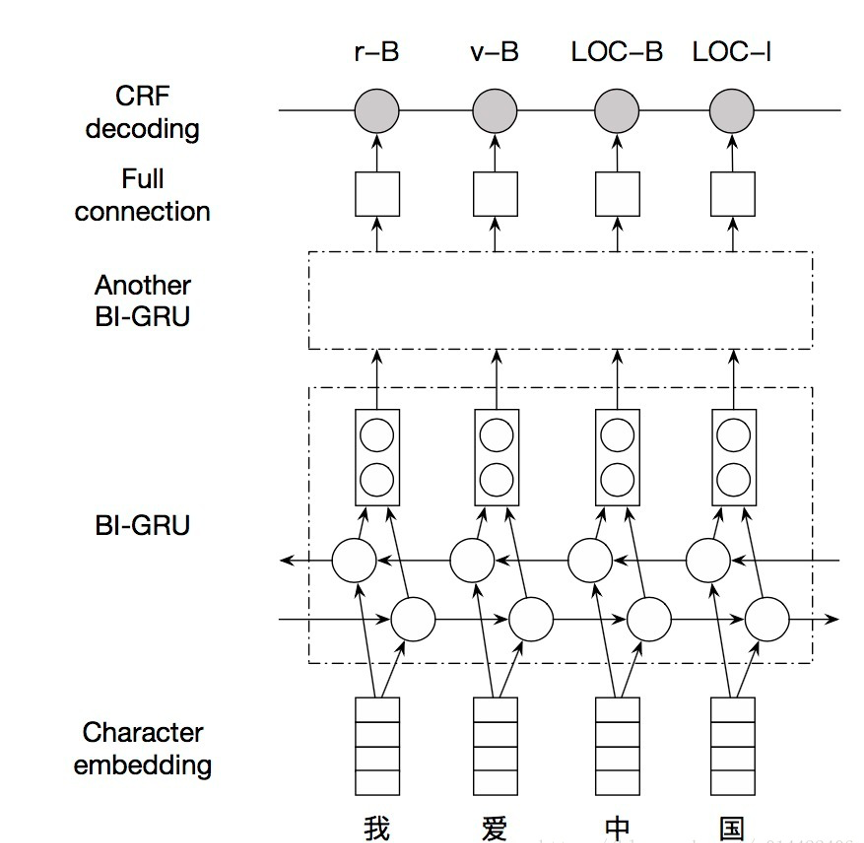
\includegraphics[scale=0.5]{bigru_crf}
  \caption{BiLSTM-CRF}
  \label{fig:bilstm_crf}
\end{figure}

数据输入部分的处理与基于字的\texttt{CRF}命名实体识别相似,同样是对于原始文本中的单字进行序列标注。训练过程采用的参数如表\ref{table:bigru_params}。

\begin{table}[h!]
  \begin{center}
  \resizebox{\columnwidth}{!}{%
  \begin{tabular}{|l|l|l|}
  \hline \textbf{参数} & \textbf{解释} & \textbf{数值} \\ \hline
    batch\_size & batch大小 & 256  \\
    hidden\_dim & GRU层单元数 & 256 \\
    epochs & 数据迭代次数 & 100 \\
    embedding\_dim & 词嵌入层维数 & 300 \\
    embedding\_lr & 词嵌入层学习率 & 1 \\
    crf\_lr & CRF层学习率 & 0.2 \\
    bigru\_num & 双向GRU单元数 & 2 \\
    learning\_rate & 总学习率 & 0.001 \\
    clip & 梯度裁剪阈值 & 5.0 \\
    dropout\_rate & 网络单元失活率 & 0.2 \\
    updata\_embedding & 词嵌入层更新 & True \\
  \hline
  \end{tabular}
  }
  \end{center}
  \caption{\label{table:bigru_params} \texttt{BiGRU-CRF}参数 }
\end{table}

\subsubsection{基于\texttt{ERNIE}的命名实体识别}
预训练模型在NLP领域目前较多任务均有较好的表现效果,预训练模型的核心思想为借助深度学习模型复杂的结构和强大的非线性表示学习能力,学习到海量数据中存在的本质(知识),
把这些知识以向量或者参数的形式存储起来,并通过feature或者parameter sharing的形式迁移到其他相关的领域中。

本实验过程中我们尝试了采用预训练模型来做Fine-Tuning。具体地,我们尝试使用百度推出的\texttt{ERNIE}\cite{sun2019ernie}预训练模型完成实验,在中文的命名实体识别以及文本分类问题上,
\texttt{ERNIE}的表现效果均优于\texttt{BERT}、\texttt{XLNET}等众多预训练模型。

\texttt{ERNIE}模型由两个堆叠的模块构成:

\paragraph{底层的文本编码器(T-Encoder)} 负责获取输入 token 的词法和句法信息

\paragraph{上层的知识型编码器(K-Encoder)} 负责将额外的面向 token 的知识信息整合进来自底层的文本信息

因此\texttt{ERNIE}可以在一个统一的特征空间中表征 token 和实体的异构信息了。其模型结构如图\ref{fig:ernie}\cite{sun2019ernie}。

\begin{figure*}[!h]
  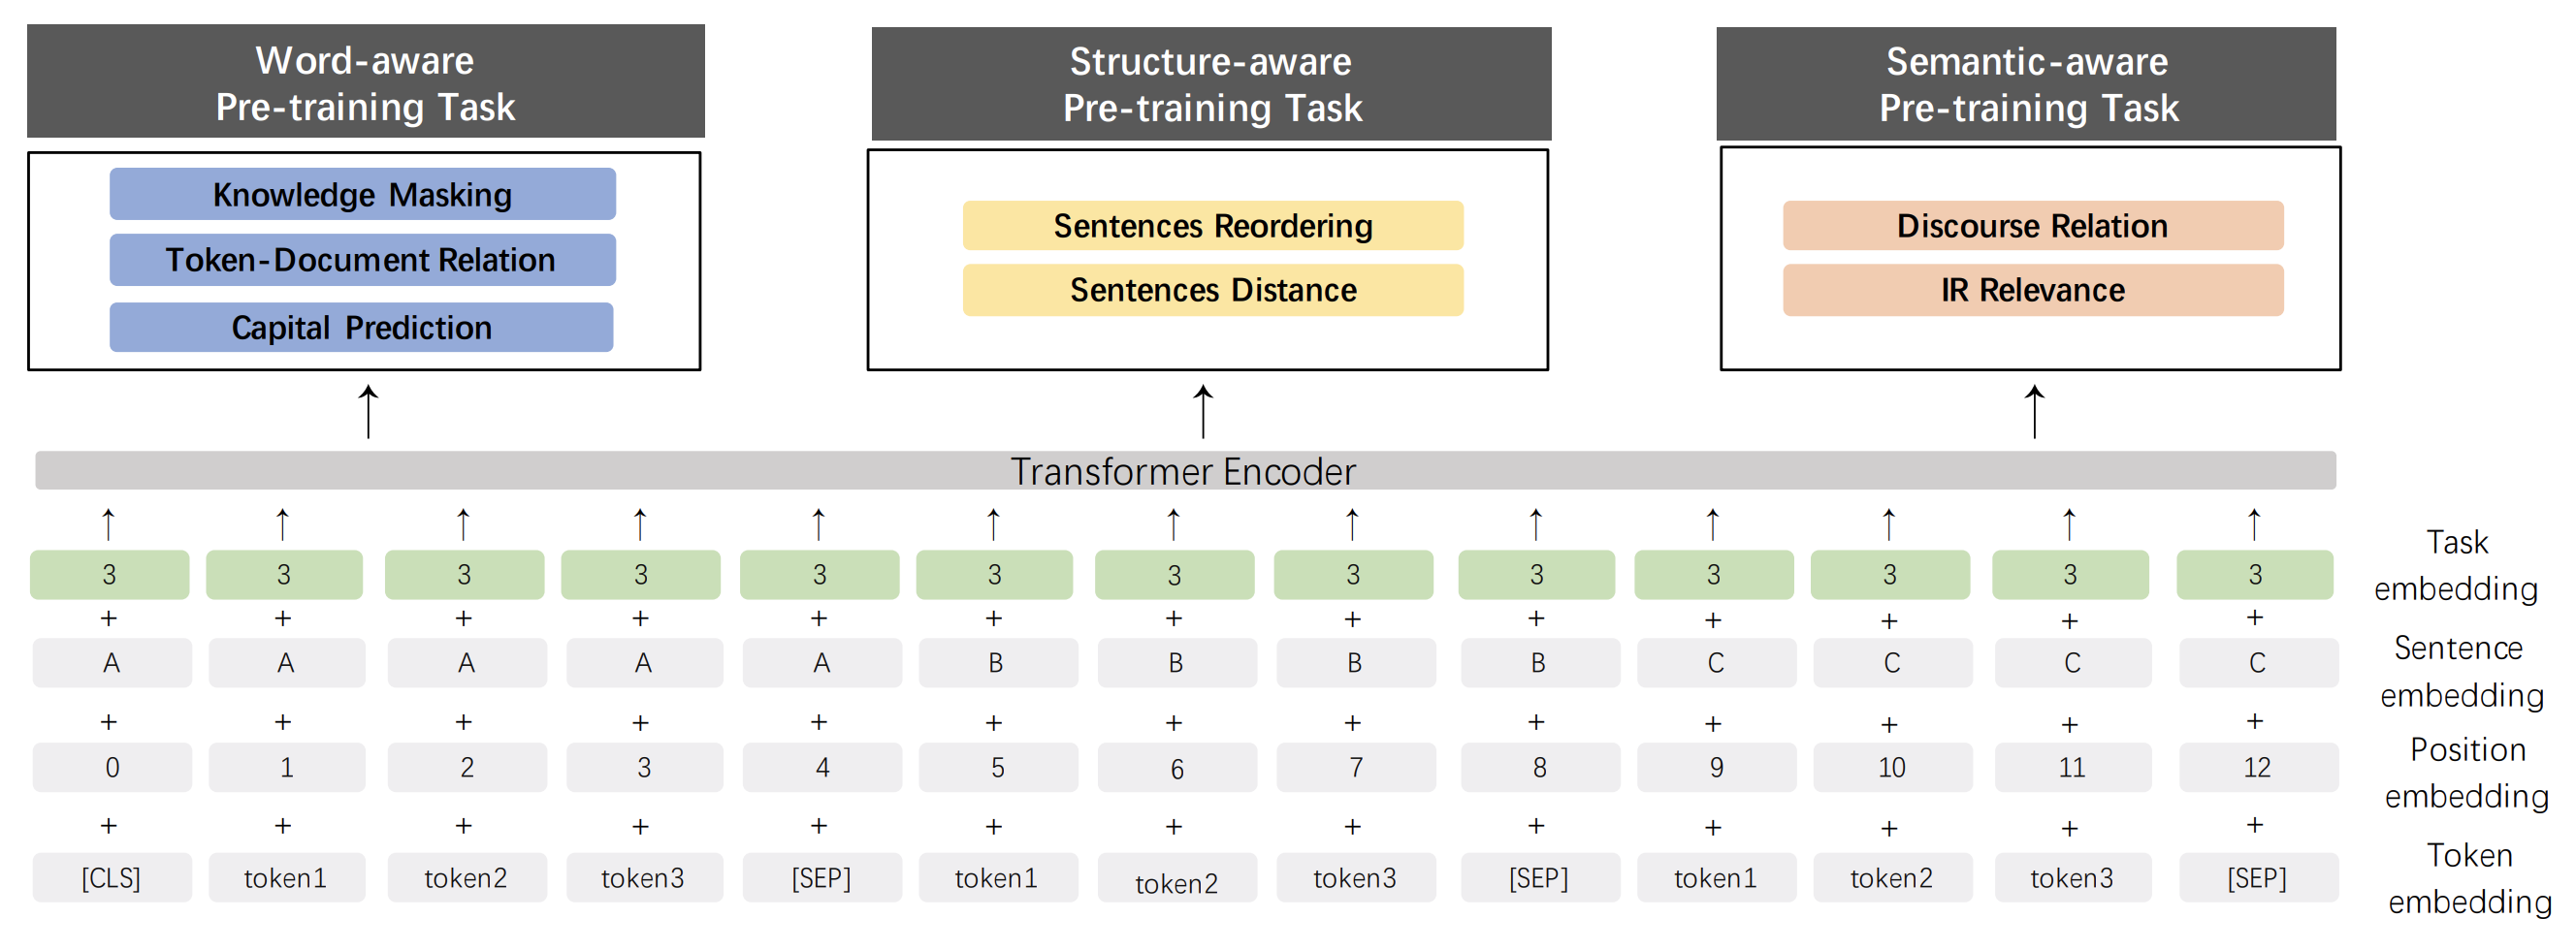
\includegraphics[scale=0.34]{ernie}
  \caption{ \texttt{ERNIE 2.0}模型结构。 输入的嵌入包含\texttt{token embedding},\texttt{sentence embedding},
\texttt{position embedding}和\texttt{task embedding}。 在此基础上,构建了七个属于不同种类的预训练任务。}
  \label{fig:ernie}
\end{figure*}

在属性词情感词提取任务中我们使用了\texttt{ERNIE}进行序列标注。数据的处理与\texttt{BiGRU-CRF}方案相似,训练参数见表\ref{table:ernie_params}。
\begin{table}[h!]
  \begin{center}
  \resizebox{\columnwidth}{!}{
  \begin{tabular}{|l|l|l|}
  \hline \textbf{参数} & \textbf{解释} & \textbf{数值} \\ \hline
    batch\_size & batch大小 & 32  \\
    weight\_decay & 权值衰减 & 0.01 \\
    num\_epoch & epoch数 & 200 \\
    max\_seq\_len & 最大序列长度 & 128 \\
    learning\_rate & 学习率 & 5e-5 \\
  \hline
  \end{tabular}
  }
  \end{center}
  \caption{\label{table:ernie_params} \texttt{ERNIE}参数 }
\end{table}

在采用\texttt{ERNIE}进行序列标注时,我们统计了训练集的标注,发现属性词情感词中包含非汉字的只有6个实例,如“\texttt{挺OK的}”,只占总数据量的$0.015\%$,因此我们
针对非汉字字符对数据集和测试集进行数据清洗,以获得更好的效果。
我们的清洗工作包括:

\begin{itemize}
  \item 替换文中空格为全角逗号
  \item 去除句末非汉字的字符
  \item 去除句中所有非实体且非汉字且非常规标点集的字符
  \item 连续同一个标点符号替换为单个标点符号
\end{itemize}

此外,我们尝试了进行数据增强,我们将训练集句子拆分为子句,并随机以\texttt{Bigram}或\texttt{Trigram}方式拼接这些子句,得到的新数据集为原数据集大小的$1.5$倍。

\subsection{属性词-情感词关系配对}

我们统计了训练集中的数据,发现6633条评论中仅有72条评论的属性词和情感词位于不同的子句中(即属性词和观点词之间存在逗号或句号),占总数据的$1.09\%$,
因此在进行关系配对时,我们\textbf{假设所有的属性词和情感词均位于一个子句中},以此减小不合理的搭配数。我们采用了两种方法来进行关系配对,分别是基于栈的关系配对和基于深度学习的关系配对。
为了简化表述,下文中属性词简记为\texttt{F},情感词简记为\texttt{O}。

\subsubsection{基于栈的属性词-情感词配对}
分析训练集,可以发现商品评论的属性词-情感词分布较为简单:主要为\texttt{F-O}、\texttt{O-F}和单独的\texttt{O}。同时由于在上文统计中假设了所有的属性词和情感词位于一个子句中,
这使得单纯基于栈的属性词-情感词关系匹配具有一定的合理性。
算法描述为:按序扫描每个子句中的属性词与情感词,如果栈为空或者当前词与栈顶词类别相同,则将当前词压入栈;如果当前词与栈顶词类别不同,则弹栈,栈顶词与当前词组成一个关系对;如果扫描完了子句中的
所有词且栈非空,则将栈中的每一个词单独作为一个一元关系。下文结果分析中会发现这种简单的方式实际效果较好。

\subsubsection{基于\texttt{ERNIE}的属性词-情感词配对}
在自然语言处理中,处理预定义关系抽取的一种做法是将其转化为分类问题:枚举命名实体关系对,并判断它们是否为预定义的关系\cite{zeng2014relation}。在此问题中,预定义关系即为属性词-情感词对,
因此可以采用上述分类方法完成配对任务。具体地,我们采用了\texttt{ERNIE}预训练模型的句对分类任务来实现这一目标。我们抽取了所有的标记中的二元非空属性词情感词关系对用作训练集的正例,一共有1655条;
又在每一句评论中抽取了所有的非正例的二元非空属性词情感词对用作训练集的负例,一共有723条;然后按照$0.7:0.15:0.15$的比例划分数据集测试集训练集进行训练。
我们先后尝试了两种输入模式:

\begin{itemize}
  \item 属性词、情感词直接作为输入的句对进行句对分类任务。
  \item 原句作为句对中的第一句,属性词与情感词在添加分隔符连接到一起后作为句对中的第二句。如“\texttt{这次快递真快}”,输入为“\texttt{这次快递真快, 快递|真快}”。
\end{itemize}

特别地,我们尝试了从不同的句子中抽取非正例的二元非空属性词情感词用作负例以平衡正例和负例的比例至$1655:1655$,但实际匹配效果要差于初始的数据非均衡的情况。

最后,我们还分析了配对结果,发现其中包含57个有一个实体为单字的属性词-情感词对,且这部分单字不出现在训练集中的实体中。我们认为这属于明显不正确的结果,并基于规则筛除了这部分结果。

\subsection{属性分类}

属性分类任务中,由于只有13个预定义的类别,这一问题可以被认为是文本单分类问题。在之前的属性词-情感词配对任务中我们认识到了预训练模型\texttt{ERNIE}的强大。
我们认为借助其复杂的模型结构和在大量语料上学到的知识,可以在属性分类这一文本单分类问题上取得不错的结果。因而我们直接采用了\texttt{ERNIE}进行这一步骤的文本分类任务。
我们将训练集标记中的属性词-情感词拼接成单句,并采用\texttt{ERNIE}的单句分类任务模型进行分类。

\subsection{观点极性分类}

观点极性分类任务只有\texttt{正面}、\texttt{中性}和\texttt{负面}三个类别,因而实质上也是一个文本单分类问题。我们采用了类似上一步骤属性分类的做法,将属性词与情感词拼接,
并采用\texttt{ERNIE}的单句分类任务进行分类。

\section{实验结果}

\subsection{属性词情感词命名实体识别与关系配对}
我们首先分别采用基于词的\texttt{CRF}、基于字的\texttt{CRF}、\texttt{biGRU+CRF}和\texttt{ERNIE}进行命名实体识别,并采用基于栈的属性词-情感词配对。

对于\texttt{CRF}方案,我们按$0.9:0.1$划分训练集测试集,在测试集上计算序列标注的$F1$值(忽略\texttt{OFF}标记)。
基于词的\texttt{CRF}在测试集上的$F1$值达到了$0.8522$,而基于字的\texttt{CRF}则达到了$0.9672$。
进行属性词-情感词配对之后,在CodaLab平台上基于词的\texttt{CRF}得分为$0.7520$,而基于字的\texttt{CRF}得分为$0.7664$。

我们随后抛弃训练集,使用所有数据训练模型并提交CodaLab平台,基于词的\texttt{CRF}得分下降了,而基于字的\texttt{CRF}得分上升为$0.7772$。
$0.7772$也是我们采用传统机器学习方案达到的最高分。

对于深度学习进行序列标注的方案,我们按$0.7:0.15:0.15$划分训练集、测试集和验证集。

采用\texttt{BiGRU-CRF}进行序列标注的方案,在训练100个epoch过后,提交成绩为$0.64$,训练200个eopch后成绩提升为$0.68$,训练400个epoch后效果达到$0.7112$,为此方案最终结果。

而采用\texttt{ERNIE}进行序列标注的方案,在没有采用数据清洗的情况下,模型在验证集上的$F1$值达到了$0.85$,此时上交得到的得分为$0.7957$,
超过了其它所有方案的得分。我们随后对原数据进行了数据清洗,模型在验证集上的$F1$值达到了$0.89$,此时上交得分为$0.8171$。

我们随后尝试了采用\texttt{ERNIE}进行属性词-情感词配对任务。
我们采用的两种方案,\texttt{直接将属性词、情感词作为句对进行分类},和\texttt{将原句、用分隔符连接的属性词情感词作为句对进行分类},均取得了较基于栈的方案更高的得分。
其中第一种方案在CodaLab得到了$0.8219$的分数,而第二种方案达到了$0.8261$。

值得注意的是,我们尝试了使用增强过的数据训练\texttt{ERNIE}的序列标注模型,尽管在本地验证集上的$F1$值上升了数个百分点,提交得分有所下降。

我们将本地训练集数据舍去,而只采用训练集和验证集,在第一个任务得分为$0.8289$。

最后我们基于规则筛除了结果中明显有问题的属性词-情感词对,最终在第一个任务得分\textbf{0.8317}。

\subsection{属性分类}
我们采用基于\texttt{ERNIE}单句分类任务模型进行训练,在训练了7个epoch后在本地验证集上的$F1$值达到了$0.95$,此时利用上一步骤提取的属性词-观点词对进行分类,
在CodaLab上得到了$0.7893$的分数。我们随后在属性词情感词命名实体识别上进行了改进,最终这一任务的得分为\textbf{0.8040}。

\subsection{观点极性分类}
观点极性分类我们同样采用了\texttt{ERNIE}单句分类任务模型进行训练,在训练了7个epoch后在本地验证集的$F1$值达到了$0.97$,此时利用第一步提出的属性词-观点词对进行分类,
在CodaLab上得到了$0.7751$的分数。在投入精力改进了第一个任务的结果之后,最终这一任务得分为\textbf{0.7899}。

\subsection{实验结果汇总}
我们在每个任务采用不同模型所达到的最终得分见表\ref{table:score}。

\begin{table}[!h]
  \centering
  \begin{tabular}{|p{1.7cm}|c|c|}
  \hline \textbf{任务} & \textbf{模型} & \textbf{F1值}  \\ \hline
  \multirow{4}{1.7cm}{属性词-情感词识别} & 基于词的\texttt{CRF} & 0.7550 \\ \cline{2-3}
  & 基于字的\texttt{CRF} & 	0.7772 \\ \cline{2-3}
  & \texttt{BiGRU-CRF} & 0.7112 \\ \cline{2-3}
  & \texttt{ERNIE}序列标注模型 & \textbf{0.8317} \\ \hline
  属性分类 & \texttt{ERNIE}单句分类模型 & \textbf{0.8040} \\ \hline
  观点极性分类 & \texttt{ERNIE}单句分类模型 & \textbf{0.7899} \\ 
  \hline
  \end{tabular}
  \caption{\label{table:score} 最终各模型在CodaLab上得分 }
\end{table}


\section{实验结果分析}

\subsection{属性词情感词命名实体识别}
从上述实验结果可以得到,在属性词-情感词提取问题上,总体上基于字的\texttt{CRF}效果要好于基于词的\texttt{CRF},两种\texttt{CRF}效果在给定数据集上的效果要好于\texttt{BiGRU-CRF};
而预训练模型\texttt{ERNIE}的效果要明显好于其它方法。

这样的结果与预期有所不符:首先利用了更多信息的基于词的\texttt{CRF}效果没有好于单纯基于字的\texttt{CRF},其次深度学习中的\texttt{BiGRU-CRF}方案效果差于两种\texttt{CRF}方案。

对于第一个问题的一种解释是,基于词的\texttt{CRF}需要用到分词信息、词性和依存句法,这些信息是通过\texttt{pkuseg}和\texttt{LTP工具}得出的。商品评论较为口语化且包含众多网络用语,而\texttt{LTP工具}训练所使用的语料为人民日报,
因而词性分析和依存句法分析效果不理想。而基于字的\texttt{CRF}虽然利用的信息相对于基于词的\texttt{CRF}更少,但却也不需要使用预处理工具得的中间结果,也就不存在误差累计问题。这是基于字的\texttt{CRF}表现更好的原因。

\texttt{BiGRU-CRF}模型相比于\texttt{CRF}模型能够更充分地利用上下文信息,但同时它的参数空间较大,需要较大的语料进行训练。实验中所使用语料只有3229条评论,6634条属性词-情感词关系对。这个数据量较小,因而用于训练\texttt{BiGRU-CRF}模型效果一般。
相比之下,\texttt{ERNIE}预训练模型在模型更加复杂、能够更好利用上下文信息的同时,已经在大规模语料下进行了训练,在此实验中的序列标注任务中仅仅进行了fine-tuning,因而不仅需要的语料更小,而且表现效果也较好。

另外,我们所做的数据增强工作均表现为负优化,我们认为这是由于采用\texttt{EDA}所使用的替换词典与此领域相关性较弱,此外子句拼接引入了不当的噪声。

\subsection{属性词-情感词关系配对}
由于\texttt{ERNIE}利用了语义信息所以显然效果要好于基于栈的机械配对。
而我们在采用\texttt{ERNIE}进行属性词-情感词关系配对时所采用单两种方案表现不同,其中\textit{将原句作为句对中的第一句,属性词与情感词在添加分隔符连接到一起后作为句对中的第二句}的方案由于在属性情感词关系对的基础上利用了句子上下文的信息,
因而效果要好于单纯\textit{将属性词、情感词直接作为输入的句对进行句对分类任务}的方案。

\subsection{属性分类}
我们在属性分类上采用\texttt{ERNIE}进行单句分类,采用第一个任务得分$0.8171$的结果即达到了$0.7892$。这相当于分类任务的\texttt{ACC}达到了$0.9658$。

\subsection{观点极性分类}
我们在观点极性分类上采用\texttt{ERNIE}进行单句分类,同样采用前两个任务得分$0.8171$的结果即达到了$0.7751$,相对于第二个任务下降了$0.0141$。这相当于第三问分类任务的\texttt{ACC}达到了$0.9821$。结合第二个任务属性分类的结果,我们认为实验的改进空间
主要为第一个任务,因此我们随后将工作中心转移到了提升命名实体识别精确率和属性观点匹配的精确率上。

\section{实验心得体会与致谢}
本次实验分为了三个部分,我们在属性词情感词抽取部分投入了较多的精力,实验的方法从基于字、词的\texttt{CRF}到深度学习再到预训练模型,我们学习到了不同的特征对\texttt{CRF}性能的影响,
实践了深度学习中各种参数的调整策略、神经网络的组织方法与输入层的的数据表示等深度学习基本问题,将课堂知识成功运用到实验中,加深了对课堂的理解。预训练模型的使用,让我们接触到当前NLP最前沿的科技成果,通过学习预训练模型,我们深深地为工业机器的强大所折服。

完成实验与论文撰写的过程充满了挑战与艰辛,实施过程中遇到很多难以解决的问题,使评价对象及属性词抽取模型性能较低。但是在小组成员通力合作下,我们查阅了许多论文与实现方法,将问题逐一击破,完成了实验各部分的任务指标。
在这里,我们特别感谢我们的授课老师——孙承杰老师,他在我们实验完成过程及论文撰写上提供了很多建议和指导,并在我们实验过程中启发式的引导思路,让我们更好的理解实验内容,我们实验最终得以完成,与孙承杰老师的指导与帮助是离不开的。
同时我们要感谢这次实验中的两位助教,他们帮助我们分析了\texttt{ERNIE}模型训练中的异常情况,并启发了我们采用\texttt{ERNIE}完成属性词-观点词的配对任务。
以本次实验为契机,我们接触到了中文自然语言处理的基础问题——命名实体识别以及文本分类,从多个技术实现路线尝试解决命名实体识别任务,对自然语言处理中统计模型、深度学习方法以及预训练模型有了直接的认识,并提高了实践能力和解决问题的能力。
通过接触各种统计模型与实现技术,我们也感到了自然语言处理的博大精深,相信在之后的学习中,我们会继续努力,争取更大的进步。

\section{贡献分权重分配}
牟虹霖\ 1173710132\ \textbf{1}

侯鹏钰\ 1173710217\ \textbf{0.95}

\bibliography{acl2019}
\bibliographystyle{acl_natbib}

\end{document}
